\documentclass[../main.tex]{subfiles}
\begin{document}
\chapter{Matrix Groups}
\section{General and Special Linear Groups}
Let $M_n(\R)$ be the set of $n \times n$ matrices with real entries.
From Vectors and Matrices we know that matrix multiplication is associative and the identity matrix provides an identity for matrix multiplication.
However, not all matrices are invertible, recall that:
\begin{lemma}
  A matrix $A \in M_n(\R)$ has an inverse if and only if $\det A \neq 0$.
\end{lemma}
\begin{proof}
  See Vectors and Matrices 3.5.1
\end{proof}
\begin{definition}[General Linear Group]
  The \textit{General Linear Group} is defined as:
  \[
    \GL_n(\R) = \{A \in M_n(\R) : \det A \neq 0\}
  \]
  This is a group by the above discussion.
\end{definition}
\begin{lemma}
  For matrices $A, B \in M_n(\R)$:
  \[
    \det(AB) = \det A \det B
  \]
\end{lemma}
\begin{proof}
  See Vectors and Matrices 3.5.5
\end{proof}
This means that $\det$ is a homomorphism:
\[
  \det: \GL_n(\R) \to \R_\times,\ A \mapsto \det A
\]
\begin{remark}[Notation]
  $\R_\times$ is the group of $(\R \setminus \{0\}, 1, \times)$ under multiplication.
\end{remark}
\begin{definition}[Special Linear Group]
  The \textit{special linear group} is defined to be:
  \begin{align*}
    \SL_n(\R) &= \ker(\det) \\
              &= \{A \in M_n(\R) : \det A = 1\}
  \end{align*}
\end{definition}
Since $\SL_n$ is the kernel of a homomorphism, it must be a normal subgroup of $\GL_n$, that is:
\[
  \SL_n(\R) \lhd \GL_n(\R)
\]
So by the Isomorphism Theorem (\cref{isomorphismTheorem}), we have:
\[
  \GL_n(\R) / \SL_n(\R) \cong \im (\det)
\]
Consider following determinant for any $x \in \R_\times$:
\[
  \det \begin{pmatrix}
  x & 0 & \cdots & 0 & 0 \\
  0 & 1 & \cdots & 0 & 0 \\
  \vdots & \vdots & \ddots & \vdots & \vdots \\
  0 & 0 & \cdots & 1 &  0\\
  0 & 0 & \cdots & 0 & 1 \\
  \end{pmatrix} =
  \det \left(\begin{array}{c|c}
    x & O \\ \hline
    O & I
  \end{array}\right) = x
\]
Therefore, $\im(\det) = \R_\times$ so:
\[
  \GL_n(\R)/\SL_n(\R) = \R_\times
\]

All of the above makes just as much sense when $\R$ is replaced with $\C$ so we also have:
\[
  \GL_n(\C) \text{ and } \SL_n(\C)
\]
and again:
\[
  \GL_n(\C) / \SL_n(\C) \cong \C_\times
\]
\section{Change of Basis}
There is a natural action of $\GL_n(\R)$ on $M_n(\R)$ by conjugation, that is:
\[
  \GL_n(\R) \acts M_n(\R) \text{ by } P(A) = PAP^{-1}
\]
\begin{proposition}
  Let $V$ be an $n$ dimensional vector space (over $\R$) and $\alpha: V \to V$ a linear map.
  If $A \in M_n(\R)$ that represents $\alpha$ in some basis, then the orbit:
  \[
    GL_n(\R)A = \{PAP^{-1} : P \in \GL_n(\R)\}
  \]
  consists of \textbf{all} the matrices that represent $\alpha$ in any basis.
\end{proposition}
\begin{proof}
  \begin{proofdirection}{Suppose a matrix $B$ represents $\alpha$ in some basis}
    A basis $\{\vec{v}_1, \ldots, \vec{v}_n\}$ for $V$ defines an isomorphism of vector spaces:
    \[
      \phi: \R^{n} \to V,\ (\lambda_1, \ldots, \lambda_n) \mapsto \sum_{i = 1}^{n} \lambda_i \vec{v}_i
    \]
    This relation between $\R^{n}$ and $V$ can be expressed diagrammatically:
    \begin{center}
    \begin{tikzcd}
    \R^n \arrow{d}[swap]{A} \arrow{r}{\phi}[swap]{\cong} & V \arrow{d}{\alpha} \\
    \R^n \arrow{r}{\phi}[swap]{\cong} & V
    \end{tikzcd}
    \end{center}
    The claim that $A$ represents $\alpha$ in this basis means that:
    \[
      \alpha = \phi A \phi^{-1}
    \]
    Likewise, another basis  $\{\vec{u}_1, \ldots, \vec{u}_n\}$ corresponds to another isomorphism $\psi: \R^{n} \to V$, and a matrix $B$ represents $\alpha$ in these coordinates if $B = \psi^{-1} \alpha \psi \iff \alpha = \psi B \psi^{-1}$.

    Therefore:
    \begin{align*}
      B &= \psi^{-1} \alpha \psi \\
        &= (\psi^{-1} \circ \phi) A (\phi^{-1} \circ \psi) \\
        &= PAP^{-1}
    \end{align*}
    where $P \in \GL_n(\R)$ represents:
    \[
      \psi^{-1} \circ \phi: \R^{n} \to \R^{n}
    \]
    in the standard basis.
    We know that $P \in GL_n(\R)$ as we know that it has an inverse given by the matrix representing $\phi^{-1} \circ \psi$.

    So $B \in \GL_n(\R)A$.
    Thus, the set of all matrices representing $\alpha$ is contained in the orbit.
  \end{proofdirection}
  \begin{proofdirection}{Suppose a matrix $B$ is in the orbit of $A$}
    Conversely, if $B = PAP^{-1}$, for some $P \in \GL_n(\R)$, then by setting:
    \[
      \psi = \phi \circ P^{-1}: \R^{n} \to V
    \]
    we get a basis $\{\vec{u}_i = \psi(\vec{e}_i)\}$ for $V$.
    In this basis, $B$ represents $\alpha$.

    Thus the orbit is contained in the set of matrices representing $\alpha$
  \end{proofdirection}
\end{proof}
\section{M\"obius Transformations Revisited}
Recall from \cref{mobComposition} that multiplication in $\mob$ looked similar to multiplication of $2 \times 2$ matrices.
Now that we have studied quotient groups in \cref{quotientGroups}, we can more precisely describe this relation using a quotient group.
\begin{proposition}
  If we identify $\C_\times$ with the following diagonal $2 \times 2$ matrices in $\GL_2(\C)$:
  \[
    \C_{\times} = \left\{ \lambda I = \begin{pmatrix}
    \lambda & 0 \\
    0 & \lambda \\
    \end{pmatrix} \in \GL_2(\C) : \lambda \in \C \setminus \{0\} \right\}
  \]
  Then $\C_\times \lhd \GL_2(\C)$ and:
  \[
    \mob \cong \GL_2(\C)/\C_\times
  \]
\end{proposition}
\begin{proof}
  Define the map $\Phi: \GL_2(\C) \to \mob$ as:
  \[
    \begin{pmatrix}
    a & b \\
    c & d \\
    \end{pmatrix} \mapsto
    \left(z \mapsto \frac{az + b}{cz + d}\right)
  \]
  By our computation of multiplication in \cref{mobComposition}, we see that $\Phi$ is a homomorphism.
  We can also see that it is surjective as if $M \in \GL_2(\C)$, $\det M = ad - bc \neq 0$, which is exactly the restriction on $a, b, c, d$ for a M\"obius transform.
  Thus, $\im \Phi = \mob$.

  A matrix $M \in \ker \Phi$ if and only if $\Phi(M) = \id$.
  From \cref{threePointMob}, we know a transform is the identity if and only if its image fixes 0, 1 and $\infty$.
  A transform fixes 0, 1 and $\infty$ if and only if:
  \[
    b = c = 0 \text{ and } a = d
  \]
  So $\ker \Phi$ is exactly the matrices in $\C_\times$.
  Since $\ker \Phi \lhd \GL_2(\C)$, we have $\C_\times \lhd \GL_2(\C)$.
  Finally, by the Isomorphism Theorem (\cref{isomorphismTheorem}), we have $M \cong \GL_2 /\C_\times$.
\end{proof}
\section{Orthogonal Groups}
\subsection{Orthogonal Group}
We want to do geometry using special types of matrices so we need to define a notion of distance.
We will denote the usual euclidean norm in $\R^{n}$ as $\norm{\cdot}$, defined as:
\[
  \norm{\vec{u}} = \sqrt{\sum_{i=1}^{n} u^{2}_{i}}
\]
\begin{definition}[Orthogonal Group]
  The \textit{$n$-dimensional orthogonal group}, $O(n),$ is the subgroup of $\GL_n(\R)$ that preserves distance in $\R^{n}$.
  That is:
  \[
    O(n) = \{A \in \GL_n(\R): \norm{A \vec{v}} = \norm{\vec{v}} \text{ for all } \vec{v} \in \R^{n}\}
  \]
\end{definition}
The dot product:
\[
  \vec{u} \cdot \vec{v} = \sum_{i = 1}^{n} u_i v_i
\]
is often more convenient to work with as it encodes information about both lengths and angles.
We can show that $O(n)$ is equivalently only the matrices that preserve the dot product.
We first need a simple but useful lemma:
\begin{lemma}[Polarisiation Identity]
  For any vectors $\vec{u}, \vec{v} \in \R^{n}$,
  \[
    2(\vec{u} \cdot \vec{v}) = \norm{\vec{u}}^2 + \norm{\vec{v}}^2 - \norm{\vec{u} - \vec{v}}^2
  \]
\end{lemma}
\begin{proof}
  \begin{align*}
    \norm{\vec{u} - \vec{v}}^2 &= (\vec{u} - \vec{v}) \cdot (\vec{u} - \vec{v}) \\
                            &= \norm{\vec{u}}^2 - 2(\vec{u} \cdot \vec{v}) + \norm{\vec{v}}^2
  \end{align*}
  From which the result follows.
\end{proof}
We can now characterise $O(n)$ using the dot product:
\begin{lemma}[$O(n)$ and Dot Products]
  \[
    O(n) = \{A \in \GL_n(\R) : (A\vec{x}) \cdot (A\vec{y}) = \vec{x} \cdot \vec{y} \text{ for all } \vec{x}, \vec{y} \in \R^{n}\}
  \]
  That is, $O(n)$ is the set of all matrices that preserves the dot product.
\end{lemma}
\begin{proof}
  If $A \in \GL_n(\R)$ preserves the dot product, then $(A\vec{x})\cdot(A\vec{y}) = \vec{x} \cdot \vec{y}$ for all $\vec{x} , \vec{y} \in \R^{n}$.

  For any $v \in \R^{n}$, we then have:
  \begin{align*}
    \norm{A \vec{v}}^2 &= (A \vec{v}) \cdot (A \vec{v}) \\
                    &= \vec{v} \cdot \vec{v} \\
                    &= \norm{\vec{v}}^2
  \end{align*}
  Thus $\norm{A \vec{v}} = \norm{\vec{v}}$ so $A \in O(n)$

  Conversely, if $A \in O(n)$, then for any $\vec{x} , \vec{y} \in \R^{n}$ then:
  \begin{align*}
    2(A \vec{x}) \cdot (A \vec{y}) &= \norm{A\vec{x}}^2 + \norm{A\vec{y}}^2 - \norm{A\vec{x} - A\vec{y}}^2 \text{ (by polarisation identity)}\\
                                   &= \norm{A\vec{x}}^2 + \norm{A\vec{y}}^2 - \norm{A(\vec{x} - \vec{y})}^2 \\
                                   &= \norm{\vec{x}}^2 + \norm{\vec{y}}^2 - \norm{\vec{x} - \vec{y}}^2 \text{ (as $A \in O(n)$))}\\
                                   &= 2(\vec{x} \cdot \vec{y}) \text{ (by polarisation identity)}
  \end{align*}
  Thus $(A\vec{x})\cdot(A \vec{y}) = \vec{x} \cdot \vec{y}$ so $A$ preserves the dot product.
  Therefore both characterisations of $O(n)$ are equivalent.
\end{proof}
This quickly leads to a nice characterisation of matrices in $O(n)$:
\begin{lemma}[Matrices in $O(n)$]
  Let $A \in M_n(\R)$.
  The following statements are equivalent:
  \begin{enumerate}
    \item $A \in O(n)$
    \item The columns of $A$ form an orthonormal basis for $\R^{n}$.
    \item $A^{\trans} A = I$
  \end{enumerate}
\end{lemma}
\begin{proof}
  Let $A = (a_{i j})$.

  (\textbf{i} $\implies$ \textbf{ii})\par
  \begin{indentenvironment}
    Let $\{\vec{e}_1, \ldots, \vec{e}_n\}$ be the standard basis for $\R^{n}$.
    The $i$-th column of $A$ is the column vector $A \vec{e}_i$.
    Since $A \in O(n)$ we have:
    \[
      (A\vec{e}_i) \cdot (A\vec{e}_j) = \vec{e}_i \cdot \vec{e}_j = \delta_{i j}
    \]
    which is exactly what it means for the columns of $A$ to form an orthonormal basis.
  \end{indentenvironment}

  (\textbf{ii} $\implies$ \textbf{iii})\par
  \begin{indentenvironment}
    As explained above, \textbf{ii} means that:
    \[
      (A\vec{e}_i) \cdot (A\vec{e}_j) = \delta_{i j}
    \]
    Since $\vec{u} \cdot \vec{v} = \vec{u}^{\trans} \vec{v}$, this means that:
    \begin{align*}
      (A\vec{e}_i)^{\trans} (A\vec{e}_j) &= \delta_{i j} \\
      \vec{e}^{\trans}_{i} A^{\trans} A \vec{e}_j &= \delta_{i j}
    \end{align*}
    But $\vec{e}^{\trans}_{i}M\vec{e}_j = M_{i j}$, so $(A^{\trans}A)_{i j} = \delta_{i j}$.
    Thus $A^{\trans} A = I$.
  \end{indentenvironment}

  (\textbf{iii} $\implies$ \textbf{i})\par
  \begin{indentenvironment}
    Suppose $\vec{u}, \vec{v} \in \R^{n}$.
    Then:
    \begin{align*}
      (A \vec{u}) \cdot (A \vec{v}) &= (A \vec{u})^{\trans} (A \vec{v}) \\
                                    &= \vec{u}^{\trans} A^{\trans} A \vec{v} \\
                                    &= \vec{u}^{\trans} I \vec{v} \text{ (as $A^{\trans} A = I$)} \\
                                    &= \vec{u}^{\trans} \vec{v} \\
                                    &= \vec{u} \cdot \vec{v}
    \end{align*}
    So $A \in O(n)$, as required.
  \end{indentenvironment}
\end{proof}
Recall from Vectors and Matrices 3.5.5 that $\det A^{\trans} = \det A$.
Therefore:
\[
  1 = \det I = \det(A^{\trans} A) = \det A^{\trans} \det A = (\det A)^2
\]
So $\det A = \pm 1$ for any $A \in O(n)$.
\subsection{Special Orthogonal Group}
\begin{definition}[Special Orthogonal Group]
  We define the \textit{special orthogonal group} as:
  \begin{align*}
    \SO(n) &= O(n) \cap \SL_n(\R) \\
           &= \{A \in O(n) : \det A = 1\}
  \end{align*}
\end{definition}
Note that:
\[
  \SO(n) = \ker(\det: O(n) \to \{\pm 1\})
\]
So $\SO \lhd O(n)$.
Furthermore, since we know that there are orthogonal matrices with $\det A = -1$, we have that $|O(n):\SO(n)| = 2$.
Examples of orthogonal matrices with $\det A = -1$, i.e. those in $O(n) \setminus \SO(n)$, are provided by \textit{reflections}.
\subsection{Reflections and Rotations}
\begin{definition}[Reflections]
  Any $\vec{v} \in \R^{n} \setminus \{\vec{0}\}$ defines an \textit{orthogonal plane}:
  \[
    P_{\vec{v}} = \{x \in \R^{n}: \vec{x} \cdot \vec{v} = 0\}
  \]
  The \textit{reflection} in the plane $P_{\vec{v}}$ is defined to be:
  \[
    S_{\vec{v}}(\vec{x}) = \vec{x} - 2 \frac{(\vec{x} \cdot \vec{v})}{\norm{\vec{v}}^2} \vec{v}
  \]
\end{definition}
\begin{remark}[Remarks]
  \begin{enumerate}
    \item We will sometimes write $S_P$ for reflection in the plane $P$.
    \item We may replace $\vec{v}$ by $\frac{\vec{v}}{\norm{\vec{v}}}$ and assume that $\norm{\vec{v}} = 1$ for simplicity so that $S_{\vec{v}}$ becomes:
      \[
        S_{\vec{v}}(\vec{x}) = \vec{x} - 2(\vec{x} \cdot \vec{v})\vec{v}
      \]
  \end{enumerate}
\end{remark}
\begin{lemma}
  $S^2_{\vec{v}} = I$ and $S_{\vec{v}} \in O(n)$
\end{lemma}
\begin{proof}
  We may assume that $\norm{\vec{v}} = 1$.
  Note that $S_{\vec{v}}$ is linear in $\vec{x}$ so has a matrix representation $S_{\vec{v}} \in M_n(\R)$.

  Consider the dot product:
  \begin{align*}
    (S_{\vec{v}}(\vec{x}) \cdot \vec{v}) &= (\vec{x} \cdot \vec{v}) - 2(\vec{x} \cdot \vec{v})\underbrace{(\vec{v} \cdot \vec{v})}_{=1} \\
                                         &= - (\vec{x} \cdot \vec{v})
  \end{align*}
  Therefore when we compute $S^{2}_{\vec{v}}(\vec{x})$, we get:
  \begin{align*}
    S^{2}_{\vec{v}}(\vec{x}) &= S_{\vec{v}}(\vec{x}) - 2(S_{\vec{v}}(\vec{x}) \cdot \vec{v})\vec{v} \\
                             &= \vec{x} - 2(\vec{x} \cdot \vec{v})\vec{v} + 2(\vec{x} \cdot \vec{v}) \vec{v} \\
                             &= \vec{x}
  \end{align*}
  So indeed $S^{2}_{\vec{v}} = I$.
  This also means that $S_{\vec{v}}$ is is invertible so $S_{\vec{v}} \in \GL_n(\R)$.

  Finally, for any $\vec{x} \in \R^{n}$:
  \begin{align*}
    \norm{S_{\vec{v}}(\vec{x})}^2 &= (\vec{x} - 2(\vec{x} \cdot \vec{v})\vec{v}) \cdot (\vec{x} - 2(\vec{x} \cdot \vec{v})\vec{v}) \\
                                  &= \norm{\vec{x}}^2 - 4(\vec{x} \cdot \vec{v})^2 + 4(\vec{x} \cdot \vec{v})^2 \underbrace{(\vec{v} \cdot \vec{v})}_{=1} \\
                                  &= \norm{\vec{x}}^2
  \end{align*}
  so $S_{\vec{v}}(\vec{x})$ preserves distances, thus $S_{\vec{v}}(\vec{x}) \in O(n)$.
\end{proof}
\begin{remark}
  Let $\norm{\vec{v}} = 1$ and pick an orthonormal basis $\{\vec{v}_1, \ldots, \vec{v}_{n - 1}\}$ for $P_{\vec{v}}$.
  If we adjoin $\vec{v}$ to this basis, we will get as basis $\{\vec{v}_1, \ldots, \vec{v}_{n - 1}, \vec{v}\}$ for $\R^{n}$ as $\vec{v}$ is by definition orthogonal to $P_{\vec{v}}$.

  Under a reflection, the components on the plane themselves are preserved but the component perpendicular (parallel to $\vec{v}$) is reflected so under this basis $S_{\vec{v}}$ has matrix:
  \[
    S_{\vec{v}} = \begin{pmatrix}
      1 & 0 & \cdots & 0 & 0\\
      0 & 1 & \cdots & 0 & 0 \\
      \vdots & \vdots & \ddots & \vdots & \vdots \\
      0 & 0 & \cdots & 1 & 0\\
      0 & 0 & \cdots & 0& -1 \\
    \end{pmatrix} \implies \det S_{\vec{v}} = - \det I = -1
  \]
  Since similar matrices always have the same determinant $S_{\vec{v}}$ has the same determinant in all bases, thus $\det S_{\vec{v}} = -1$ and $S_{\vec{v}} \notin \SO(n)$.
\end{remark}
\begin{theorem}[Reflections Generate $O(n)$]
  \label{reflectionsGenerate}
  Every $A \in O(n)$ is a product of \textbf{at most} $n$ reflections.
\end{theorem}
\begin{proof}
  \induction
  {$n = 1$}{
    $O(1)$ is the set of $1 \times 1$ matrices such that the columns form an orthonormal bases for $\R$.
    This means that $O(1)$ consists only of $\pm 1$ and is therefore generated by $S_{1}$.
    Thus:
    \[
      O(1) = \{\pm 1\} = \langle S_1 \rangle \cong C_2
    \]
  }
  {$n - 1$}{
    So any $A \in O(n - 1)$ can be written as a product of at most $n - 1$ reflections.
  }
  {$n$}{
    Let $\{\vec{e}_1, \ldots, \vec{e}_n\}$ be the standard basis for $\R^{n}$.
    Let $\vec{v} = \vec{e}_n - A \vec{e}_n$.
    For now, assume that $A\vec{e}_n \neq \vec{e}_n \iff \vec{v} \neq \vec{0}$ so that $P_{\vec{v}}$ is well defined.
    This is the vector that joins $\vec{e}_n$ and $A\vec{e}_n$ so we see that reflection in $P_{\vec{v}}$ will send $A\vec{e}_n$ back to $\vec{e}_n$.
    \begin{center}
    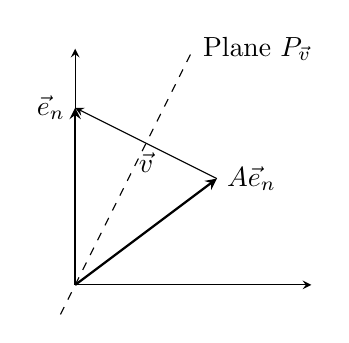
\begin{tikzpicture}[>=stealth, scale=1.5]
      \draw[->] (0, 0) -- (0, 2);
      \draw[->] (0, 0) -- (2, 0);
      \draw[->, thick] (0, 0) -- (0, 1.5) node[left] {$\vec{e}_n$};
      \draw[->, thick] (0, 0) -- (1.2, 0.9) node[right] {$A\vec{e}_n$};
      \draw[->] (1.2, 0.9) -- (0, 1.5) node[midway, below] {$\vec{v}$};
      \draw[dashed] (-0.125, -0.25) -- (1, 2) node[right] {Plane $P_{\vec{v}}$};
    \end{tikzpicture}
    \end{center}
    That is:
    \[
      (S_{\vec{v}}A)\vec{e}_n = \vec{e}_n
    \]
    So $S_{\vec{v}}A$ is an orthogonal transformation that preserves $\vec{e}_n$.
    Since orthogonal transformations preserve the dot product, so the plane $P_{\vec{e}_n}$ orthogonal to $\vec{e}_n$ must also be preserved.
    The plane $P_{\vec{e}_n} = \R^{n - 1} \times \{0\}$ as it is just all the vectors where the $n$-th component is 0.

    If we restrict $S_{\vec{v}}A$ to $P_{\vec{e}_n}$, it is still an orthogonal transformation, so, by the induction hypothesis, there exists $\vec{v}_1, \ldots, \vec{v}_{n - 1} \in \R^{n - 1} \setminus \{\vec{0}\}$ such that:
    \[
      S_{\vec{v}}A = S_{\vec{v}_1} \cdots S_{\vec{v}_{n - 1}} \text{ on }\R^{n - 1}
    \]
    Since both sides also fix $\vec{e}_n$, they must also agree on $\R^{n}$.
    Therefore $S_{\vec{v}}A = S_{\vec{v}_1} \cdots S_{\vec{v}_{n - 1}}$ and so $A = S_{\vec{v}} S_{\vec{v}_1} \cdots S_{\vec{v}_{n - 1}}$.
    Thus $A$ is a product of at most $n$ reflections.

    If $A\vec{e}_n = \vec{e}_n$, then by a similar argument using $\R^{n - 1}$, $A = S_{\vec{v}_1} \cdots S_{\vec{v}_{n - 1}}$ which is less than $n$ reflections.
  }
\end{proof}
Orthogonal transformations are especially easy to analyse in low dimensions.
\begin{lemma}[Elements of $O(2)$]
  Let $A \in O(2)$.
  \begin{enumerate}
    \item If $A \notin \SO(2)$, then $A$ is a reflection.
    \item If $A \in \SO(2)$, then $A$ is a rotation about the origin.
  \end{enumerate}
\end{lemma}
\begin{proof}
  Recall that $\det S_{\vec{v}} = -1$ so:
  \[
    \det(S_{\vec{v}_1} \cdots S_{\vec{v}_k}) = (-1)^{k}
  \]
  By \cref{reflectionsGenerate}, we may take $k \leq 2$ as $A$ can be written as a product of at most 2 reflections.

  \begin{enumerate}
    \item If $A \notin \SO(2)$, then $\det A \neq 1$ so $k$ is odd.
      Therefore $k = 1$ and therefore $A$ is just a single reflection.
    \item If $A \in \SO(2)$, then $\det A = 1$ so $k$ is even.
      Therefore, unless $A = I$, we can write $A = S_{\vec{u}} S_{\vec{v}}$ for some $\vec{u}, \vec{v}$ that are \textbf{not} parallel (otherwise they are the same reflection).

      Excluding the identity transformation, rotations fix only the origin.
      So we claim that $A = S_{\vec{u}} S_{\vec{v}}$ only fixes $\vec{0}$.

      Suppose that some $\vec{x} \neq \vec{0}$ is fixed by $A$.
      That is:
      \[
        S_{\vec{u}}S_{\vec{v}}\vec{x} = \vec{x} \iff S_{\vec{u}} \vec{x} = S_{\vec{v}}\vec{x} \iff (\vec{x} \cdot \vec{u})\vec{u} = (\vec{x} \cdot \vec{v})\vec{v}
      \]
      However, since $\vec{x}, \vec{u}, \vec{v}$ are non-zero, we conclude that $\vec{u}$ and $\vec{v}$ are parallel which is a contradiction.
      Hence $A$ only fixes $\vec{0}$ as claimed and so is a rotation about the origin.
  \end{enumerate}
\end{proof}
\begin{remark}
  Let $A \in \SO(2)$.
  We have seen that the columns form an orthonormal basis, so $A$ must be in the form:
  \[
    A = \begin{pmatrix}
    a & b \\
    -b & a \\
    \end{pmatrix}
  \]
  with $\det A = a^2 + b^2 = 1$.
  Then $a = \cos \theta$ and $b = \sin \theta$ for some $\theta$ so:
  \[
    A = \begin{pmatrix}
    \cos \theta & \sin \theta \\
    -\sin \theta & \cos \theta \\
    \end{pmatrix}
  \]
\end{remark}
\begin{lemma}[Elements of $\SO(3)$]
  If $A \in \SO(3)$, then $A$ is a rotation.
\end{lemma}
\begin{proof}
  By \cref{reflectionsGenerate}, $A$ is a product of at most 3 reflections.
  We also have $\det A = (-1)^{k}$ where $k$ is the number of reflections $A$ is composed of.

  We need $\det A = 1$ so ether $k = 0 \text{ or } 2$ and therefore either $A = I$ or $A = S_{\vec{u}}S_{\vec{v}}$ for some non-parallel $\vec{u}, \vec{v}$.

  If $A = I$ then we are done, otherwise since $n = 3$ and $\vec{u}, \vec{v}$ are non-parallel, the planes $P_{\vec{u}}$ and $P_{\vec{v}}$ must intersect in a line:
  \[
    P_{\vec{u}} \cap P_{\vec{v}} = \ell
  \]
  Both reflections fix their corresponding plane so the composition must fix their intersection thus $A$ must fix $\ell$.

  For $A$ to be a non-identity rotation, it must fix \textbf{only} the line $\ell$.
  Suppose some $\vec{x} \notin \ell$ is fixed by $A$, as in the previous lemma, that is:
  \[
    S_{\vec{u}}S_{\vec{v}}\vec{x} = \vec{x} \iff S_{\vec{u}} \vec{x} = S_{\vec{v}}\vec{x} \iff (\vec{x} \cdot \vec{u})\vec{u} = (\vec{x} \cdot \vec{v})\vec{v}
  \]
  Since $x \notin \ell = P_{\vec{u}} \cap P_{\vec{v}}$, at least one of $\vec{x} \cdot \vec{u}$ and $\vec{x} \cdot \vec{v}$ must be non-zero.
  If exactly one is non-zero then either $\vec{u} = \vec{0}$ or $\vec{v} = \vec{0}$, which is a contradiction.
  Thus both must be non-zero so we conclude that $\vec{u}$ and $\vec{v}$ are parallel which is a contradiction.
  Hence $A$ only fixes the line $\ell$ and therefore must be a rotation with axis $\ell$.
\end{proof}
\end{document}
